\documentclass{article}

% Language setting
% Replace `english' with e.g. `spanish' to change the document language
%\usepackage[english]{babel}

% Set page size and margins
% Replace `letterpaper' with`a4paper' for UK/EU standard size
\usepackage[letterpaper,top=2cm,bottom=2cm,left=3cm,right=3cm,marginparwidth=1.75cm]{geometry}

% Useful packages
\usepackage{amsmath}
\usepackage{graphicx}
\usepackage[colorlinks=true, allcolors=blue]{hyperref}

% Number sets
\usepackage{amsfonts}

\usepackage{pdfpages}

\title{TMA4115 - Matematikk 3}
\author{Magne Tenstad}

\begin{document}

\maketitle

\clearpage

\tableofcontents




\clearpage
\section{Komplekse tall}
Finner du ikke det du ser etter? Se \href{https://www.math.ntnu.no/emner/TMA4110/2020h/notater/1-komplekse-tall.pdf}{Wiki}.


\subsection{Den imaginære enheten}
Vi definerer den imaginære enheten $i$, ved
\[ i^2 = -1 \]
Merk at $ \sqrt{ab} = \sqrt{a} \, \sqrt{b} $ bare gjelder for $a, b > 0$.
\\\\
Komplekse tall er tall på formen
\[ z = a + bi \]
der $a, b \in \mathbb{R}$, og $i$ er den imaginære enheten.
\\\\
Mengden av komplekse tall er $\mathbb{C}$.


\subsection{Operasjoner på komplekse tall}
Regneregler for komplekse tall følger regnereglene for reelle tall.
\\\\
\textbf{Definisjon.} La $z = a + bi$ være et komplekst tall. Da er $z$ \textit{konjugert} gitt ved
\[ z = a - bi \]
Merk at $z\overline{z} = a^2 + b^2$ er et reelt tall.


\subsection{Polare koordinater}
Polarkoordinater er nyttige når en multipliserer og tar potenser av komplekse tall.
\\\\
La $r$ være avstanden fra det komplekse tallet $z =
a + bi$ til origo, og la $\theta$ være vinkelen $z$ gjør med den reelle aksen. Da har vi at
\begin{gather*}
    a = \text{Re}\, z = r \, \cos{\theta} \\
    b = \text{Im}\, z = r \, \sin{\theta}
\end{gather*}
$r$ kalles \textit{modulus} eller \textit{absoluttverdi} til $z$ og $\theta$ kalles \textit{vinkelen} eller \textit{argumentet} til $z$.
\begin{gather*}
    r = |z| = \sqrt{a^2 + b^2} = \sqrt{z\overline{z}} \\\\
    \theta =
    \begin{cases}
        \arctan \frac{b}{a} & \text{for } a > 0 \\
        \arctan \frac{b}{a} + \pi & \text{for } a < 0 \\
        \pi / 2 & \text{for } a = 0, \, b > 0 \\
        3\pi / 2 & \text{for } a = 0, \, b < 0 \\
    \end{cases}
\end{gather*}


\subsubsection{Trekantulikheten}
\textbf{Teorem 1.5.} La $z$ og $w$ være komplekse tall. Da gjelder at
\[ |z + w| \leq |z| + |w| \]


\subsection{Eulers formel}
Eulers formel er gitt ved
\[ e^{ix} = \cos{x} + i \, \sin{x} \]
der $x \in \mathbb{R}$ og $i$ er den imaginære enheten.
\\\\
Det følger at
\[ z = r(\cos{\theta} + i \, \sin{\theta}) = re^{i\theta} \]
\textbf{Teorem 1.7.} La $z = re^{i\theta}$ og $w = se^{i\alpha}$. Da gjelder:
\begin{align*}
    z \cdot w &= rse^{i(\theta + \alpha)} \\
    \frac{z}{w} &= \frac{r}{s} e^{i(\theta - \alpha)}
\end{align*}

\subsection{Røtter av komplekse tall}
Et polynom $f(z) = z^n + a_{z-1}z^{n-1} + ... + a_1<+a_0$, $z \in \mathbb{C}$ kan alltid faktoriseres
\[f(z) = \prod_{i=1}^n (z - z_i)\]
der $z_i \in \mathbb{C}$ er løsninger av likningen $f(z) = 0$.




\clearpage
\section{Lineære likningssystemer og gausseliminasjon}
Finner du ikke det du ser etter? Se \href{https://www.math.ntnu.no/emner/TMA4110/2020h/notater/2-lineare-likningssystemer.pdf}{Wiki}.


\subsection{Ekvivalente systemer}
Vi sier at to likningssystemer er ekvivalente dersom
de har samme løsningsmengder.


\subsection{Totalmatrisen til et system}
Et lineært likningssystem med $m$ likninger og $n$ ukjente beskrives av en matrise. Denne kalles \textit{totalmatrisen} eller \textit{den utvidede matrisen} til likningssystemet. Vi lar gjerne en vertikal linje i matrisen skille venstre og høyre del av likningene.


\subsection{Radoperasjoner}
Følgende tre måter å endre en matrise på kalles \textit{radoperasjoner}:
\begin{enumerate}
    \item Gange alle tallene i en rad med det samme tallet. Dette betyr å gange en likning med et tall. Vi kan ikke gange med 0.
    \item Legge til et multiplum av en rad i en annen. Dette er å kombinere likninger til nye likninger.
    \item Bytte rekkefølge på radene. Dette er det samme som å bytte rekkefølge på likningene.
\end{enumerate}
Vi sier at to matriser er radekvivalente hvis vi kan komme fra den ene til den andre ved å utføre en eller flere radoperasjoner. Vi bruker notasjonen $M \sim N$ for å si at to matriser $M$ og $N$ er radekvivalente.
\\\\
\textbf{Teorem 2.7.} Hvis to likningssystemer har radekvivalente totalmatriser, så er de to likningssystemene ekvivalente.


\subsection{Trappeform, redusert trappeform og pivotelementer}
\textbf{Definisjon.} Tallet lengst til venstre i en rad som ikke er $0$ kalles pivotelementet for den raden. (En rad med bare nuller har ikke noe pivotelement.)
\\\\
\textbf{Definisjon.} En matrise er på trappeform dersom det ikke er annet enn $0$-ere under hvert pivotelement, og eventuelle nullrader er helt nederst.
\\\\
\textbf{Definisjon.} En matrise er på redusert trappeform hvis den er på trappeform, pivotelementene er $1$ og alle tall som står over pivotelementer er $0$.
\\\\
\textbf{Teorem 2.11.} For enhver $m \times n$-matrise $M$, finnes en $m \times n$-matrise $N$ på redusert trappeform, slik at $M$ og $N$ er radekvivalente.


\subsection{Eksistens, entydighet og parametrisering av løsninger}
For ethvert lineært likningssystem må ett av de følgende punktene være sant:
\begin{itemize}
    \item Systemet har ingen løsning: Dette skjer når vi i redusert trappeform har en rad av typen $ 0 \ 0 \ ... \ 0 \ | \ b $ der $b \neq 0$.
    \item Systemet har entydig løsning. Dette skjer når trappeform av totalmatrisen har pivotelement i alle kolonner unntatt den siste.
    \item Systemet har uendelig mange løsninger. Dette skjer når vi får frie variabler. Vi får en fri variabel for hver kolonne (unntatt den siste) som ikke har pivotelement.
\end{itemize}


\subsection{Lineære likninger med komplekse tall}
Et lineært likningssett med komplekse koeffisienter og løsning, kan løses med gausseliminasjon på samme måte som i det reelle tilfellet.




\clearpage
\section{Vektorlikninger}
Finner du ikke det du ser etter? Se \href{https://www.math.ntnu.no/emner/TMA4110/2020h/notater/3-vektor-og-matriselikninger.pdf}{Wiki}.


\subsection{Vektorregning}
En lineærkombinasjon av vektorene $x$ og $y$ er en vektor på formen
\[ax + by\]
der $a$ og $b$ er skalarer, kalt vekter.
\\\\
Det lineære spennet til $x$ og $y$ er mengden av \textit{alle lineærkombinasjoner} av $x$ og $y$.


\subsection{Vektorlikninger}
Likningssystemer kan ofte skrives om til vektorlikninger.


\subsection{Geometrisk tolkning av vektorlikninger: Eksistens og entydighet av løsninger}
Vi tar utgangspunkt i vektorlikningen
\[ xv_1 + yv_2 + zv_3 = v_4 \]
Vi skal nå gi noen geometriske illustrasjoner i $\mathbb{R}^3$ av hva som skjer i de ulike tilfellene:
\begin{itemize}
    \item Systemet har ingen løsning: $v_4 \notin \text{Sp}\{v_1, v_2, v_3\}$
    \item Systemet har entydig løsning: $v_4 \in \text{Sp}\{v_1, v_2, v_3\}$ og $v_1, v_2, v_3$ er lineært uavhengige.
    \item Systemet har uendelig mange løsninger: $v_4 \in \text{Sp}\{v_1, v_2, v_3\}$ og $v_1, v_2, v_3$ er lineært avhengige.
\end{itemize}




\clearpage
\section{Matriser}
Finner du ikke det du ser etter? Se \href{https://www.math.ntnu.no/emner/TMA4110/2020h/notater/4-matriser.pdf}{Wiki}.


\subsection{Definisjoner og notasjon}


\subsection{Produkt av matrise og vektor}
\textbf{Teorem 4.6.} Hvis $A$ er en $m \times n$-matrise, $v$ og $w$ er vektorer i $\mathbb{R}^n$ og $c$ er en skalar, så har vi følgende likheter:
\[ A(v + w) = Av + Aw \]
\[ A(cv) = c(Av) \]


\subsection{Sum og skalering av matriser}
\textbf{Teorem 4.9.} Hvis $A$ og $B$ er $m \times n$-matriser, $v$ er en vektorer i $\mathbb{R}^n$ og $c$ er en skalar, så har vi følgende likheter:
\[ (A + B)v = Av + Bv \]
\[ (cA)v = c(Av) \]


\subsection{Matrisemultiplikasjon}
\textbf{Definisjon.} La A være en $m \times n$-matrise med rader
$a_1, a_2, \dots, a_m$, og la B være en $n \times p$-matrise med
kolonner $b_1, b_2, \dots, b_p$. Produktet av A og B er definert ved:
\[ AB = \begin{bmatrix}
a_1b_1 & a_1b_2 & \cdots & a_1b_p \\
a_1b_1 & a_1b_2 & \cdots & a_1b_p \\
\vdots & \vdots & \ddots & \vdots \\
a_mb_1 & a_mb_2 & \cdots & a_mb_p \\
\end{bmatrix} \]
\textbf{Teorem 4.13.} La $A$, $B$, og $C$ være matriser, $v$ en vektor, og $c$ et tall. I hver del av teoremet antar vi at størrelsene på matrisene og vektoren er slik at alle operasjonene som brukes er definert.\\\\
(a) Matrisemultiplikasjon er en assosiativ operasjon, det vil si:
\[ A(BC) = (AB)C \]
Et spesialtilfelle av dette er følgende:
\[ (AB)v = A(Bv) \]
(b) Å skalere et matriseprodukt er det samme som å skalene én av faktorene og deretter multiplisere:
\[ (cA)B = c(AB) = A(cB) \]
(c) Matrisemultiplikasjon distribuerer over addisjon av matriser, det vil si:
\[ A(B+C) = AB + AC \]
\[ (A + B)C = AC +\ BC \]


\subsection{Transponering}
Operasjonen \textit{transponering} går ut på å bytte om rader og kolonner.
\\\\
\textbf{Teorem 4.15.} For enhver matrise $A$ har vi:
\[ (A^\top)^\top = A \]
Hvis $A$ og $B$ er matriser slik at produktet $AB$ er definert, så er:
\[ (AB)^\top = B^\top A^\top \]


\subsection{Identitetsmatriser}
La $I = I_n$ være den kvadratiske $n \times n$-matrisen
\[ I_n = \begin{bmatrix}
1 & 0 & \cdots & 0 \\
0 & 1 & \cdots & 0 \\
\vdots & \vdots & \ddots & \vdots \\
0 & 0 & \cdots & 1
\end{bmatrix} \]
Da er $IA = A$ for enhver $n \times p$-matrise $A$ og $BI = B$ for enhver $m \times n$-matrise $B$. Spesielt er $Ix = x$ for enhver vektor $x$. Derfor kalles $I = I_n$ en identitetsmatrise, eller en $n \times n$-identitetsmatrise.


\subsection{Potenser av matriser}
Hvis $A$ er en kvadratisk matrise, så kan vi gange $A$ med seg selv. Generelt definerer vi at $A$ opphøyd i $n$-te er produktet av $A$ med seg selv $n$ ganger:
\[ A^n = A \cdot A \cdot \cdots \cdot A \]
For tall har vi definert at $a^0 = 1$. For kvadratiske matriser har vi derimot
\[ A^0 = I_n \]


\subsection{Inverser}
\textbf{Definisjon.} La $A$ være en $n \times $-matrise. En \textit{invers} til $A$ er en $n \times n$-matrise $B$ som er slik at
\[ A \cdot B = I_n = B \cdot A \]
En matrise er \textit{inverterbar} hvis den har en invers.
\\\\
\textbf{Teorem 4.18.} Hvis en matrise er inverterbar, så har den nøyaktig én invers.
\\\\
\textbf{Teorem 4.20.} La $A$ være en $n \times n$-matrise, og $b$ en vektor. Hvis $A$ er inverterbar, så har likningen $Ax = b$ entydig løsning, og løsningen er $x = A^{-1}b$.


\subsection{Beregning av inverser}
\textbf{Teorem 4.25.} La $A$ være en $n \times n$-matrise.\\\\
(a) $A$ er inverterbar hvis og bare hvis $A \sim I_n$.
\\\\
(b) Hvis $A$ er inverterbar, så kan vi finne inversen ved å gausseliminere matrisen
\[ \begin{bmatrix} A \ | \ I_n \end{bmatrix} \]
til redusert trappeform og lese av høyre halvdel av den resulterende matrisen. Med andre ord: Resultatet av gausseliminasjonen blir følgende matrise: 
\[ \begin{bmatrix} I_n \ | \ A^{-1} \end{bmatrix} \]

\subsection{Formel for invertering av $2 \times 2$-matrise}
La
\[ A = \begin{bmatrix} a & b \\ c & d \end{bmatrix} \]
Da er
\[ A^{-1} = \frac{1}{ad-bc} \, \begin{bmatrix} d & -b \\ -c & a \end{bmatrix} \]




\clearpage
\section{Lineær uavhengighet}
Finner du ikke det du ser etter? Se \href{https://www.math.ntnu.no/emner/TMA4110/2020h/notater/5-linear-uavhengighet.pdf}{Wiki}.


\subsection{Lineært spenn: overflødige vektorer}
Dersom en vektor $u$ ikke utvider spennet til en mengde vektorer $v_1, \cdots, v_n$ så er vektorene $u, v_1, \cdots, v_n$ lineært avhengige.


\subsection{Definisjon av lineær uavhengighet}
\textbf{Definisjon.} Vektorene $v_1, v_2, \cdots, v_n$ er lineært uavhengige dersom likningen
\[ x_1 v_1 + x_2 v_2 + \cdots + x_n v_n = 0 \]
ikke har andre løsninger enn den trivielle løsningen $x_1 = x_2 = \cdots = x_n = 0$. I motsatt tilfelle kalles de lineært avhengige.


\subsection{Lineær uavhengighet for to vektorer}
\textbf{Teorem 5.6.} To vektorer $u$ og $v$, begge ulik $0$, er lineært uavhengige hvis og bare hvis $u \neq cv$, for en skalar $c \neq 0$.


\subsection{Hvordan sjekke lineær uavhengighet?}
\textbf{Teorem 5.8.} La $A$ være en matrise. Følgende påstander er ekvivalente:
\begin{enumerate}
    \item Kolonnene i $A$ er lineært uavhengige.
    \item Likningen $Ax = 0$ har bare den trivielle løsningen $x = 0$.
    \item Vi får ingen frie variabler når vi løser $Ax = 0$.
    \item Når vi gausseliminerer $A$, får vi et pivotelement i hver kolonne.
\end{enumerate}
Teorem 5.8 gir oss en grei metode for å sjekke lineær uavhengighet. Hvis vi har vektorer
\[ v_1, v_2, \dots, v_n \]
kan vi finne ut om de er lineært uavhengige på denne måten:
\begin{enumerate}
    \item Lag en matrise $A = [ \ v_1 \ v_2 \ \dots \ v_n \ ]$ med disse vektorene som kolonner.
    \item Gausseliminer $A$ til trappeform.
    \item Hvis hver kolonne inneholder et pivotelement, er vektorene lineært uavhengige. Ellers er de lineært avhengige.
\end{enumerate}
\textbf{Teorem 5.12.} Gitt $n$ vektorer $v_1, v_2, \dots, v_n$ i $\mathbb{R}^m$ eller $\mathbb{C}^m$. Hvis \begin{enumerate}
    \item en av vektorene er en lineærkombinasjon av de andre, eller
    \item $n > m$,
\end{enumerate}
så er vektorene lineært avhengige.
\\\\
\textbf{Teorem 5.13.} Vektorene $v_1, v_2, \dots, v_n$ er lineært uavhengige hvis og bare hvis ingen av dem kan skrives som en lineærkombinasjon av de andre.


\subsection{Like mange vektorer som dimensjonen}
\textbf{Teorem 5.14.} Hvis vi har $n$ vektorer $v_1, v_2, \dots, v_n$ i $\mathbb{R}^n$, så er de lineært uavhengige hvis og bare hvis de utspenner hele $\mathbb{R}^n$, altså hvis og bare hvis
\[\text{Sp}\{v_1, v_2, \dots, v_n \} = \mathbb{R}^n \]




\clearpage
\section{Determinanter}
Finner du ikke det du ser etter? Se \href{https://www.math.ntnu.no/emner/TMA4110/2020h/notater/6-determinanter.pdf}{Wiki}.


\subsection{Determinanter for 2 x 2-matriser}
For en $2 \times 2$-matrise
\[ A = \begin{bmatrix} a & b \\ c & d \end{bmatrix} \]
er determinanten definert ved:
\[ \det{A} = \begin{vmatrix} a & b \\ c & d \end{vmatrix} = ad - bc \]
Arealet av parallellogrammet utspent av kolonnene i $A$ er lik
\[ | \det{A} | \]


\subsection{Determinanter for 3 x 3-matriser}
For en $3 \times 3$-matrise
\[ A =
\begin{bmatrix}
a_{11} & a_{12} & a_{13} \\
a_{21} & a_{22} & a_{23} \\
a_{31} & a_{32} & a_{33}
\end{bmatrix} \]
er determinanten definert ved:
\begin{align*}
    \det{A} &=
    \begin{vmatrix}
    a_{11} & a_{12} & a_{13} \\
    a_{21} & a_{22} & a_{23} \\
    a_{31} & a_{32} & a_{33}
    \end{vmatrix} \\
    &= a_{11}\begin{vmatrix} a_{22} & a_{23} \\ a_{32} & a_{33} \end{vmatrix}
    - a_{12}\begin{vmatrix} a_{21} & a_{23} \\ a_{31} & a_{33} \end{vmatrix}
    + a_{13}\begin{vmatrix} a_{21} & a_{22} \\ a_{31} & a_{32} \end{vmatrix}\\
    &= a_1 \cdot a_2 \times a_3 = |a_1|\,|a_2|\,|a_3|\,\sin{\alpha}\cos{\theta}
\end{align*}


\subsection{Determinanter og radoperasjoner}
\textbf{Teorem 6.5.} La $A$ være en $n \times n$-matrise, og la $B$ være en matrise vi får ved å utføre en radoperasjon på $A$. Da har vi følgende sammenheng mellom determinantene til $A$ og $B$, basert på hvilken type radoperasjon vi utførte:
\begin{table}[h]
    \centering
    \begin{tabular}{c|c}
        Radoperasjon & Resultat \\
        \hline 
        Gange en rad med et tall $k$ & $\det{B} = k \cdot \det{A}$ \\
        Legge til et multiplum av én rad i en annen & $\det{B} = \det{B}$ \\
        Bytte om to rader & $\det{B} = -\det{A}$
    \end{tabular}
\end{table}


\subsection{Triangulære matriser}
\textbf{Teorem 6.8.} La $A$ være en (øvre eller nedre) triangulær $n \times n$-matrise. Da er determinanten til $A$ lik produktet av tallene på diagonalen i $A$:
\[ \det{A} = a_{11} \cdot a_{22} \cdot \cdots \cdot a_{nn} \]
\textbf{Teorem fra LF} La $A$ være en øvre triangulær $n \times n$-matrise. Da er egenverdiene til $A$ elementene på diagonalen.


\subsection{Flere regneregler for determinanter}
\textbf{Teorem 6.10.} Determinanten til et produkt av to matriser er produktet av determinantene. Altså: Hvis $A$ og $B$ er to $n \times n$-matriser, så er
\[ \det{AB} = (\det{A})(\det{B}) \]
\textbf{Teorem 6.11.} Determinanten endrer seg ikke når vi transponerer matrisen. Altså: Hvis $A$ er en $n \times n$-matrise, så er
\[ \det{A} = \det{A^{\top}} \]


\subsection{Karakterisering av inverterbarhet}
\textbf{Teorem 6.12.} La $A$ være en $n \times n$-matrise. Følgende påstander er ekvivalente:
\begin{enumerate}
    \item $A$ er inverterbar.
    \item $\det{A} \neq 0$.
    \item Kolonnene i $A$ er lineært uavhengige.
    \item Kolonnene i $A$ utspenner $\mathbb{C}^n$.
\end{enumerate}




\clearpage

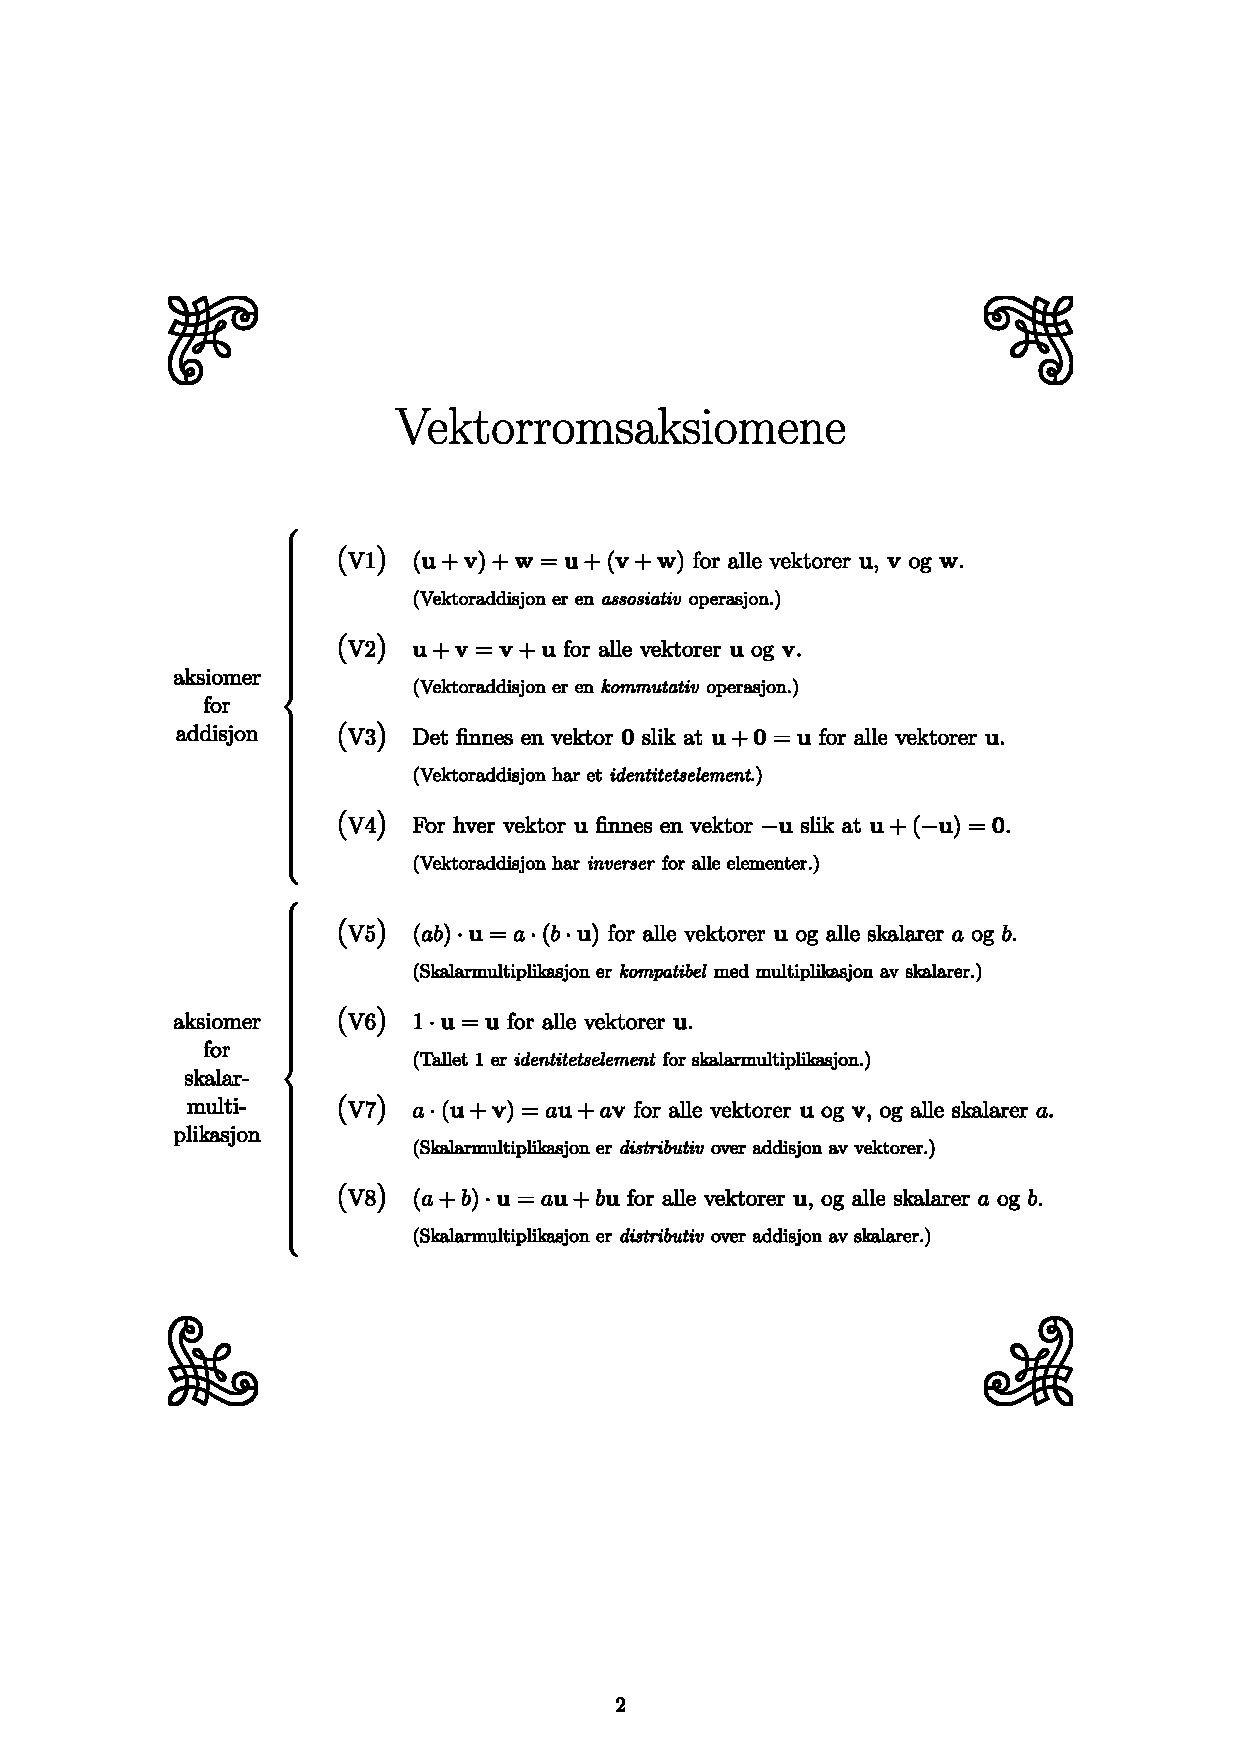
\includepdf[]{assets/vektorromaksiomene.pdf}

\section{Vektorrom}
Finner du ikke det du ser etter? Se \href{https://www.math.ntnu.no/emner/TMA4110/2020h/notater/7-vektorrom.pdf}{Wiki}.


\subsection{Definisjonen av vektorrom}
\textbf{Definisjon.} La $V$ være en mengde, og anta at vi har definert to operasjoner:
\begin{gather*}
    \text{addisjon av vektorer:} \ u + v \\
    \text{skalarmultiplikasjon:} \ c \cdot u
\end{gather*}
Addisjon skal være definert for alle elementer $u$ og $v$ i $V$, og skalarmultiplikasjonen for alle skalarer $c$ og alle $u$ i $V$. Resultatet av operasjonene skal alltid være et element i $V$. Dersom mengden $V$ og de to operasjonene oppfyller vektorromsaksiomene (V1)-(V8), så sier vi at $V$ er et \textit{vektorrom}, og vi kaller elementene i $V$ for \textit{vektorer}.


\subsection{Generelle egenskaper og lineær uavhengighet}
\textbf{Definisjon.} La $v_1, v_2, \dots, v_n$ være vektorer i vektorommet $V$. Disse vektorene er \textit{lineært} uavhengige dersom likningen
\[c_1 \cdot v_1 + c_2 \cdot v_2 + \cdots + c_n \cdot v_n = 0 \]
ikke har andre lsninger enn den trivielle løsningen $c_1 = c_2 = \cdots = c_n = 0.$ I motsatt tilfelle kalles de \textit{lineært avhengige}.
\\\\
\textbf{Teorem 7.3.} Gitt $n$ vektorer $v_1, v_2, \dots, v_n$ i et vektorrom $V$. Hvis
\begin{enumerate}
    \item en av vektorene er en lineærkombinasjon av de andre, eller
    \item en av vektorene er $0$,
\end{enumerate}
så er vektorene lineært avhengige.


\subsection{Flere eksempler på vektorrom}
\begin{itemize}
    \item Polynomer av begrenset grad.
    \item Alle polynomer.
    \item Kontinuerlige funksjoner.
    \item Deriverbare og glatte funksjoner.
    \item Matriser.
\end{itemize}


\subsection{Underrom}
\textbf{Definisjon.} Et \textit{underrom} av et vektorrom $V$ er en delmengde $U \subseteq V$ som i seg selv utgjør et vektorrom, med addisjon og skalarmultipliskasjon definert på samme måte som i $V$.
\\\\
\textbf{Teorem 7.9.} La $V$ være et vektorrom. En delmengde $U \subseteq V$ er et underrom av $V$ hvis og bare hvis følgende tre betingelser er oppfylt.
\begin{enumerate}
    \item Nullvektoren $0$ i $V$ ligger i $U$.
    \item For alle vektorer $u$ og $v$ i $U$ er også summen $u + v$ i $U$.
    \item For alle vektorer $u$ i $U$ og alle skalarer $c$ er også skalarproduktet $cu$ u $U$.
\end{enumerate}
\textbf{Teorem 7.11} En mengde $\text{Sp}\{v_1, v_2, \dots, v_n\}$ utspent av vektorer i et vektorrom $V$ er alltid et underrom av $V$.


\subsection{Endeligdimensjonale vektorrom}
\textbf{Definisjon.} Et vektorrom $V$ er \textit{endeligdimensjonalt} hvis det finnes en endelig mengde av vektorer i $V$ som utspenner $V$. Ellers er $V$ \textit{uendeligdimensjonalt}.


\subsection{Basis}
\textbf{Definisjon.} En \textit{basis} for et vektorrom $V$ er en liste
\[ B = (b_1, b_2, \dots, b_n) \]
av vektorer i $V$ som både utspenner $V$ og er lineært uavhengige.
\\\\
\textbf{Teorem 7.14.} La $V$ være et vektorrom med basis
\[ B = (b_1, b_2, \dots, b_n) \]
Da kan hver vektor $v$ i $V$ skrives som en lineærkombinasjon
\[ v = c_1b_1 + c_2b_2 + \cdots + c_nb_n \]
av basisvektorene i $B$, på en entydig måte.
\\\\
\textbf{Definisjon.} Tallene $c_1, c_2, \dots, c_n$ i teorem 7.14 kalles \textit{koordinatene} til vektoren $v$ \textit{med hensyn på} basisen $B$. Vi definerer notasjonen $[\,v\,]_B$ for vektoren i $\mathbb{C}^n$ som består av koordinatene til v:
\[ [\,v\,]_B = \begin{bmatrix}
    c_1 \\ c_2 \\ \vdots \\ c_n
\end{bmatrix} \]
\textbf{Teorem 7.16.} La $V$ være et vektorrom med basis $B$. Koordinatene til en lineærkombinasjon av vektorer er tilsvarende lineærkombinasjonen av koordinatene til hver vektor:
\[ [\, c_1v_1 + c_2v_2 + \cdots + c_tv_t\,]_B = c_1 \cdot [\,v\,]_B + c_2 \cdot [\,v_2\,]_B + \cdots + c_t \cdot [\,v_t\,]_B \]
\textbf{Teorem 7.18.} La $V$ være et endeligdimensjonalt vektorrom. Da kan enhver endelig mengde som utspenner $V$ reduseres til en basis for $V$. Mer presist: Hvis $G$ er en endelig mengde av vektorer slik at $\text{Sp}\,G = V$, så finnes en delmengde $B \subseteq G$ slik at vektorene i $B$ utgjør en basis for $V$.
\\\\
\textbf{Teorem 7.19.} Ethvert endeligdimensjonalt vektorrom har en basis.
\\\\
\textbf{Teorem 7.20.} La $V$ være et endeligdimensjonalt vektorrom. Enhver endelig mengde av vektorer i $V$ som er lineært uavhengig kan utvides til en basis. Mer presist: Hvis $L$ er en endelig mengde av vektorer som er lineært uavhengige, så finees en basis for $V$ som inneholder alle vektorene i $L$.


\subsection{Dimensjon}
\textbf{Teorem 7.21.} La $V$ være et vektorrom med en basis $B$ som består av $n$ vektorer. La $v_1, v_2, \dots, v_m$ være $m$ vektorer i $V$, der $m > n$. Da er disse vektorene lineært avhengige.
\\\\
\textbf{Teorem 7.22.} La $V$ være et endeligdimensjonalt vektorrom. Da har enhver basis for $V$ samme størrelse.
\\\\
\textbf{Definisjon.} La $V$ være et endeligdimensjonalt vektorrom. Vi definerer \textit{dimensjonen} til $V$ som antall vektorer i en basis for $V$. Vi bruker notasjonen $\dim{V}$ for dimensjonen til $V$. Hvis $B$ er en basis for $V$, har vi altså
\[ \dim{V} = |B| \]
\\\\
\textbf{Teorem 7.23.} La $V$ være et vektorrom med et underrom $U$. Hvis $V$ er endeligdimensjonalt, så er $U$ også endeligdimensjonalt, og
\[ \dim{U} \leq \dim{V} \]


\subsection{Vektorrom tilknyttet en matrise}
\textbf{Nullrommet.} Vi definerer \textit{nullrommet} til en reell $m \times n$-matrise $A$ som løsningsmengden til likningen $Ax = 0$, altså delmengden av $\mathbb{R}^n$:
\[ \text{Null}\,A = \{ x \in \mathbb{R}^n \,|\, Ax = 0 \} \]
\textbf{Kolonnerommet.} Vi definerer \textit{kolonnerommet} til en reell $m \times n$-matrise
\[ A = [\, a_1 \ a_2 \ \cdots \ a_n \,] \]
som underrommet av $\mathbb{R}^m$ utspent av kolonnene i $A$:
\[ \text{Col}\,A = \text{Sp} \{\, a_1, a_2, \dots, a_n \,\} \]
Vi kan også beskrive kolonnerommet ved
\[ \text{Col}\,A = \{\, Av \,|\, v \in \mathbb{R}^n \,\} \]
Vi finner en basis for kolonnerommet ved:
\begin{enumerate}
    \item Bruk gausseliminasjon for å finne trappeformmatrisen $A'$ som er radekvivalant til $A$.
    \item Se på $A'$ for å finne ut hvilke av kolonnene i $A$ som er pivotkolonner.
    \item Pivotkolonnene danner en basis for $\text{Col}\,A$.
\end{enumerate}
\textbf{Radrommet.} Vi definerer \textit{radrommet} til en reell $m \times n$-matrise
\[ A = \begin{bmatrix} r_1^\top \\ r_2^\top \\ \vdots \\ r_m^\top \end{bmatrix} \]
som underrommet av $\mathbb{R}^n$ utspent av radene i $A$:
\[ \text{Row}\,A = \text{Sp} \{\, r_1, r_2, \dots, r_m \,\} \]
Dette er det samme som kolonnerommet til den transponerte matrisen:
\[ \text{Row}\,A = \text{Col}\,A^\top \]
\textbf{Teorem 7.25} La $A$ være en $m \times n$-matrise, og la $E$ være trappeformmatrisen vi får når vi gausseliminerer $A$. Da har vi:
\begin{enumerate}
    \item Dimensjonen til nullrommet til $A$ er lik antall frie variabler vi får når vi løser likningssystemet $Ax = 0$, altså antall kolonner uten pivotelementer i $E$.
    \item Dimensjonen til kolonnerommet til $A$ er lik antall kolonner med pivotelementer i $E$.
    \item Dimensjonen til radrommet til $A$ er lik antall rader som ikke er null i $E$.
\end{enumerate}
\textbf{Teorem 7.26} La $A$ være en $m \times n$-matrise. Da har kolonnerommet og radommet til $A$ samme dimensjon. Dette kalles \textit{rangen} til $A$.
\[ \text{dim Col}\,A = \text{dim Row}\,A = \text{rank}\,A\]
\textbf{Teorem 7.27} La $A$ være en $m \times n$-matrise. Da er
\[ \text{dim Null}\,A + \text{rank}\,A = n \]




\clearpage
\section{Lineærtransformasjoner}
Finner du ikke det du ser etter? Se \href{https://www.math.ntnu.no/emner/TMA4110/2020h/notater/8-lineartransformasjoner.pdf}{Wiki}.


\subsection{Funksjoner}
\textbf{Definisjon.} En \textit{funksjon} består av:
\begin{enumerate}
    \item En mengde som kalles funksjonens \textit{domene}.
    \item En mengde som kalles funksjonens \textit{kodomene}.
    \item En regel som til hvert element i domenet tilordner et element i kodomenet.
\end{enumerate}
\textbf{Definisjon.} La $f: A \rightarrow B$ være en funksjon. Vi sier at $f$ er \textit{injektiv} (eller \textit{en-til-en}) hvis det for hver $b$ i $B$ er maksimalt én $a$ i $A$ slik at $f(a) = b$. Vi sier at $f$ er \textit{surjektiv} (eller \textit{på}) hvis det for hver $b$ i $B$ finnes en $a$ i $A$ slik at $f(a) = b$. \textit{Bildet} til $f$ er mengden av alle elementer i kodomenet som blir truffet av $f$, altså delmengden $\text{im} f = \{\, f(a) \ | \ a \in A \}$ av $B$.
\\\\
Det følger umiddelbart fra definisjonen at en funksjon $f: A \rightarrow B$ er surjektiv hvis og bare hvis bildet til funksjonen er hele kodomenet: $\text{im} f = B$.


\subsection{Lineærtransformasjoner}
\textbf{Definisjon.} La $V$ og $W$ være vektorrom. En funksjon $T: V \rightarrow W$ er en \textit{lineærtransformasjon} hvis den oppfyller følgende to kriterier:
\begin{enumerate}
    \item $T(u + v) = T(u) + T(v)$ for alle $u$ og $v$ i $V$.
    \item $T(cu) = c \cdot T(u)$ for alle vektorer $u$ i $V$ og alle skalarer $c$.
\end{enumerate}
\textbf{Teorem 8.3.} Hvis $T: V \rightarrow W$ er en lineærtrasformasjon, så oppfyller den følgende:
\begin{enumerate}
    \item En lineærkombinasjon i $V$ sendes til den tilsvarende lineærkombinasjonen i $W$:
    \[T(c_1v_1 + c_2v_2 + \cdots + c_rv_r) = c_1 \cdot T(v_1) + c_2 \ T(v_2) + \cdots + c_2 \cdots T(v_r) \]
    \item Nullvektoren i $V$ sendes til nullvektoren i $W$: \[ T(0) = 0 \]
\end{enumerate}
\textbf{Teorem 8.4.} La $V$ og $W$ være endeligdimensjonale vektorrom og la $T: V \rightarrow W$ være en lineærtransformasjon. Anta $B = (b_1, \dots, b_n)$ er en basis for $V$. Da er $T$ fullstendig bestemt av bildene $T(b1), \dots, T(b_n)$ av basisvektorene.


\subsection{Kjerne og bilde}
\textbf{Definisjon.} La $T: V \rightarrow W$ være en lineærtransformasjon. \textit{Kjernen} til $T$ er mengden av alle vektorer i $V$ som blir sendt til nullvektoren i $W$:
\[ \text{ker}\,T = \{\,v \in V \ | \ T(v) = 0 \} \]
\textbf{Teorem 8.8.} La $T: V \rightarrow W$ være en lineærtransformasjon.
\begin{enumerate}
    \item Kjernen $\text{ket}\,T$ er et underrom av $V$.
    \item Bildet $\text{im}\,T$ er et underrom av $W$.
\end{enumerate}
\textbf{Teorem 8.9.} En lineærtransformasjon $T: V \rightarrow W$ er injektiv hvis og bare hvis $\text{ker}\,T=\{\,0\,\}$.


\subsection{Lineærtransformasjoner gitt ved matriser}
\textbf{Teorem 8.11.} La $A$ være en $m \times n$-matrise, og la $T: \mathbb{R}^n \rightarrow \mathbb{R}^m$ være en lineærtransformasjon gitt ved $T(x) = Ax$. Da er
\[ \text{ker}\,T = \text{Null}\,A \quad \text{og} \quad \text{im}\,T=\text{Col}\,A \]
\textbf{Teorem 8.13.} La $T: \mathbb{R}^n \rightarrow \mathbb{R}^m$ være en lineærtransformasjon. Da er
\[ T(x) = Ax \quad \text{for alle } x \text{ i } \mathbb{R}^n \]
der $A$ er $m \times n$-matrisen gitt ved
\[ [ \ T(e_1) \ T(e_2) \ \cdots \ T(e_n) \ ] \]
hvor $(e_1, e_2, \dots, e_n)$ er standardmatrisen for $\mathbb{R}^n$.
\\\\
\textbf{Definisjon.} Matrisen $A$ i teorem 8.13 kalles \textit{standardmatrisen} til lineærtransformasjonen $T$.
\\\\
\textbf{Teorem 8.14.} La $T: \mathbb{R}^n \rightarrow \mathbb{R}^m$ være en lineærtransformasjon og la $A$ være standardmatrisen til $T$. Da vet vi:
\begin{enumerate}
    \item $T$ er surjektiv hvis og bare hvis kolonnene i $A$ utspenner hele $\mathbb{R}^m$.
    \item $T$ er injektiv hvis og bare hvis kolonnene i $A$ er lineært uavhengige.
\end{enumerate}


\subsection{Lineærtransformasjoner og basiser}
\textbf{Teorem 8.15.} La $V$ og $W$ være endeligdimensjonale vektorrom, og la $B$ og $C$ være basiser for henholdsvis $V$ og $W$. La $T: V \rightarrow W$ være en lineærtransformasjon. Da finnes en matrise $A$ slik at
\[ [ \ T(x) \ ]_C = A \cdot [ \ x \ ]_B \]
for alle vektorer $x$ i $V$.
\\\\
\textbf{Teorem 8.16.} La $V$ være et $n$-dimensjonalt vektorrom, og la $B = (b_1, b_2, \dots, b_n)$ og $C = (c_1, c_2, \dots, c_n)$ være to basiser for $V$. Da finnes en $n \times n$-matrise $A$ slik at
\[ [ \ x \ ]_C = A \cdot [ \ x \ ]_B \]
for alle vektorer $x$ i $V$.


\subsection{Isomorfi}
\textbf{Definisjon.} La $T: V \rightarrow W$ være en lineærtransformasjon. En \textit{invers} til $T$ er en lineærtransformasjon $S: W \rightarrow V$ som er slik at
\begin{align*}
    S(T(v)) = v \quad &\text{for alle } v \text{ i } V \text{, og} \\
    T(S(w)) = w \quad &\text{for alle } w \text{ i } W
\end{align*}
\textbf{Definisjon.} Hvis $T: V \rightarrow W$ er en lineærtransformasjon som har en invers, så er $T$ en \textit{isomorfi}. Da sier vi dessuten at vektorrommene $V$ og $W$ er \textit{isomorfe}, og vi skriver $V \cong W$.
\\\\
\textbf{Teorem 8.19.} En lineærtransformasjon er en isomorfi hvis og bare hvis den er både injektiv og surjektiv.
\\\\
\textbf{Teorem 8.22.} Hvis $V$ er et $n$-dimensjonalt komplekst vektorrom, så er $V$ isomorft med $\mathbb{C}^n$. Og hvis $W$ er et $n$-dimensjonalt reelt vektorrom, så er $W$ isomorft med $\mathbb{R}^n$.




\clearpage
\section{Projeksjon}
Finner du ikke det du ser etter? Se \href{https://www.math.ntnu.no/emner/TMA4110/2020h/notater/9-projeksjon.pdf}{Wiki}.


\subsection{Skalarproduktet i $R^n$}
\textbf{Teorem 9.3.} Den ortogonale projeksjonen på en vektor $v$,
\begin{gather*}
    P_v : \mathbb{R}^n \rightarrow \mathbb{R}^n \\
    P_v(w)=\frac{v \cdot w}{v \cdot v}\,v
\end{gather*}
er en lineærtransformasjon.


\subsection{Indreproduktrom}
\textbf{Definisjon.} La $V$ være et reelt vektorrom. Et \textit{indreproduktrom} i $V$ er en operasjon som tar inn to vektorer, $v$ og $w$, for å gi ut et reelt tall $\langle v, w \rangle$. Operasjonen tilfredsstiller
\begin{align*}
    &\langle v, w \rangle = \langle w, v \rangle &\text{(symmetri)} \\
    &\langle v, (aw + bu) \rangle = a \langle v, w \rangle + b \langle v, u \rangle &\text{(linearitet)} \\
    &\langle v, v \rangle \geq 0 \text{, og } \langle v, v \rangle = 0 \text{ kun hvis } v = 0 &\text{(positivitet)}
\end{align*}
Vi sier at $V$, sammen med et valgt indreprodukt, er et \textit{indreproduktrom}.
\\\\
\textbf{Teorem 9.6.} (Pytagoras). La $V$ være et reelt indreproduktrom. Dersom vektorene $v$ og $w$ er ortogonale, er
\[ \lVert v + w \rVert = \lVert v \rVert^2 + \lVert w \rVert^2 \]
\textbf{Teorem 9.7.} (Cauchy-Schwarz). La $V$ være et reelt indreproduktrom. Alle vektorer $v$ og $w$ tilfredstiller
\[| \langle v, w \rangle | \leq \lVert v \rVert \lVert w \rVert \]
\textbf{Teorem 9.8.} La $V$ være et indreproduktrom. Den ortogonale projeksjonen på en vektor $v$,
\begin{gather*}
    P_v : \mathbb{R}^n \rightarrow \mathbb{R}^n \\
    P_v(w)=\frac{\langle v, w \rangle}{\langle v, v \rangle}\,v
\end{gather*}
er en lineærtransformasjon.
\\\\
\textbf{Teorem 9.9.} La $v$ og $w$ være to vektorer i et indreproduktrom $V$. Da er $P_v(w)$ og $w-P_v(w)$ ortogonale.


\subsection{Ortogonal projeksjon}
\textbf{Definisjon.} En \textit{ortogonal mengde} er en mengde av ikke-null vektorer $u_1, u_2, \dots, u_n$, slik at
\[ \langle u_i, u_k \rangle = 0 \]
for alle vektorer $u_i$ og $u_k$ i mengden med $i \neq k$. Dersom i tillegg $\lVert u_j \rVert = 1$ for alle vektorene, sier vi at mengden er \textit{ortonormal}.
\\\\
\textbf{Teorem 9.10.} En ortogonal mengde er lineært uavhengig.
\\\\
\textbf{Definisjon.} Dersom en ortogonal mengde $u_1, u_2, \dots, u_n$ i $V$ også er en basis, sier vi at mengden er en \textit{ortogonal basis} for $V$.
\\\\
\textbf{Teorem 9.12.} Koordinatene til $v$ i en ortogonal basis $u_1, u_2, \dots, u_n$ er
\begin{align*}
    v &= P_{u_1}(v) + P_{u_2}(v) + \dots + P_{u_n}(v) \\
    &= \frac{\langle u_1, v \rangle}{\langle u_1, u_1 \rangle}\,u_1
    + \frac{\langle u_2, v \rangle}{\langle u_2, u_2 \rangle}\,u_2
    + \dots + \frac{\langle u_n, v \rangle}{\langle u_n, u_n \rangle}\,u_n
\end{align*}
\textbf{Teorem 9.13.} La $u_1, u_2, \dots, u_n$ være en ortogonal basis for $U$, et underrom av $V$. Punktet
\begin{align*}
    P_U(v) &= P_{u_1}(v) + P_{u_2}(v) + \dots + P_{u_n}(v) \\
    &= \frac{\langle u_1, v \rangle}{\langle u_1, u_1 \rangle}\,u_1
    + \frac{\langle u_2, v \rangle}{\langle u_2, u_2 \rangle}\,u_2
    + \dots + \frac{\langle u_n, v \rangle}{\langle u_n, u_n \rangle}\,u_n
\end{align*}
er et punktet i $U$ som har kortest avstand til $v$, altså
\[ \lVert v - P_U(v) \rVert = \text{min}_{u \in U} \lVert v - u \rVert \]
\textbf{Teorem 9.15.} La $u_1, u_2, \dots, u_n$ være en basis for et underrom $U$. En vektor $v$ er i det ortogonale komplementet til $U$ hvis og bare hvis $\langle u_i, v \rangle = 0$ for alle $i$.
\\\\
\textbf{Teorem 9.17.} La $U$ være et underrom av et indreproduktrom $V$. Da gjelder
\[ \dim{U} + \dim{U^\perp} = \dim{V} \]
\textbf{Teorem 9.18.} La $A$ være en $m \times n$-matrise. Da vet vi
\begin{align*}
    (\text{Col}\,A)^\perp &= \text{Null}\,A^T \\
    (\text{Null}\,A)^\perp &= \text{Col}\,A^T
\end{align*}


\subsection{Finne en ortogonal basis: Gram-Schmidts metode}
\textbf{Teorem 9.19.} Mengden $u_1, u_2, \dots, u_n$ gitt ved
\begin{align*}
    u_k &= v_k - \sum_{j=1}^{k-1}\,P_{u_j}(v_k) \\
    &= v_k - \sum_{j=1}^{k-1}\,\frac{\langle u_j, v_k \rangle}{\langle u_j, u_j \rangle}\,u_j
\end{align*}
er en ortogonal basis for rommet utspent av $v_1, v_2, \dots, v_n$.


\subsection{Beregne den ortogonale basisen}
La $U$ være et underrom til et indreproduktrom $V$. Her er en metode for å regne ut den ortogonale projeksjonen $P_U$:
\begin{enumerate}
    \item Ta utgangspunkt i en basis $v_1, v_2, \dots, v_n$ som spenner ut $U$.
    \item Bruk så Gram-Schmidt til å finne en ortogonal basis $u_1, u_2, \dots, u_n$ for $U$.
    \item Da kan man, for alle $v$ i $V$, beregne den ortogonale projeksjonen
    \[P_U(x) = P_{u_1}(x) + P_{u_2}(x) + \dots + P_{u_n}(x) \]
    \item Hvis $V = \mathbb{R}^n$, så får vi standardmatrisen
    \[ [\, P_U \,] = [\, P_U(e_1) \ P_U(e_2) \ \dots \ P_U(e_n) \, ] \]
    og da kan man, for alle $x$ i $V$, beregne den ortogonale projeksjonen $P_U(x) = [\, P_U \,]x$.
\end{enumerate}


\subsection{Indreproduktrom mellom funksjoner}
\textbf{Teorem 9.22.} Operasjonen
\[ \langle f, g \rangle = \frac{1}{b - a} \int_a^b f(x)\,g(x)\,dx \]
er et indreprodukt på $C([a, b])$.
\\\\
\textbf{Teorem 9.27.} Vektorene $1$, $\cos{nx}$ og $\sin{mx}$, hvor $n, m = 1, 2, 3, \dots,$ er parvis ortogonale i $C_s([-\pi, \pi])$.


\subsection{Komplekse indreprodukt}
\textbf{Definisjon.} La $V$ være et komplekst vektorrom. Et \textit{indreproduktrom} i $V$ er en operasjon som tar inn to vektorer, $v$ og $w$, for å gi ut et komplekst tall $\langle v, w \rangle$. Operasjonen tilfredsstiller
\begin{align*}
    &\langle v, w \rangle = \overline{ \langle w, v \rangle } &\text{(konj. sym.)} \\
    &\langle v, (aw + bu) \rangle = a \langle v, w \rangle + b \langle v, u \rangle &\text{(linearitet)} \\
    &\langle v, v \rangle \geq 0 \text{, og } \langle v, v \rangle = 0 \text{ kun hvis } v = 0 &\text{(positivitet)}
\end{align*}
Vi sier at $V$, sammen med et valgt indreprodukt, er et \textit{indreproduktrom}.
\\\\
\textbf{Teorem 9.29.} Alt som gjelder for reelle indreproduktrom, med unntak av vinkelen, gjelder også for komplekse indreproduktrom.
\\\\
\textbf{Teorem 9.33.} La $A$ være en kompleks $m \times n$-matrise. Da har vi
\begin{align*}
    (\text{Col}\,A)^\perp &= \text{Null}\,A^* \\
    (\text{Null}\,A)^\perp &= \text{Col}\,A^*
\end{align*}




\clearpage
\section{Egenverdier og egenvektorer}
Finner du ikke det du ser etter? Se \href{https://www.math.ntnu.no/emner/TMA4110/2020h/notater/10-egenverdier-og-egenvektorer.pdf}{Wiki}.


\subsection{Definisjon av egenverdier og egenvektorer}
\textbf{Definisjon.} La $T: V \rightarrow V$ være en lineærtransformasjon. En skalar $\lambda$ er en \textit{egenverdi} for $T$ hvis det finnes en vektor $v \neq 0$ i $V$ slik at
\[ T(v) = \lambda \cdot v \]
Vektoren $v$ kalles en \textit{egenvektor} for $T$ som hører til egenverdien $\lambda$. Når $T$ er gitt ved en $n \times n$-matrise $A$, så sier vi også at $\lambda$ er en egenverdi for $A$ og $v$ er egenvektor for $A$ som hører til egenverdien $\lambda$.


\subsection{Noen generelle observasjoner}
\textbf{Teorem 10.3.} Anta at $\lambda$ er en egenverdi for en lineærtransformasjon $T: V \rightarrow V$, og at $v$ er en tilhørende egenvektor. Da er alle multipletter $cv$ av vektoren $v$, der $c$ er et tall som ikke er $0$, også egenvektorer som hører til egenverdien $\lambda$. Med andre ord er alle vektorer i mengden $\text{Sp}\{v\}$, unntatt nullvektoren, egenvektorer som hører til egenverdien $\lambda$.
\\\\
\textbf{Teorem 10.4.} En $n \times n$-matrise $A$ har $0$ som egenverdi hvis og bare hvis den ikke er inverterbar.
\\\\
\textbf{Teorem 10.5.} La $T: V \rightarrow V$ være en lineærtransformasjon. La $v_1, v_2, \dots, v_t$ være egenvektorer til $T$ som hører til forskjellige egenverdier $\lambda_1, \lambda_2, \dots, \lambda_t$. Da er vektorene $v_1, v_2, \dots, v_t$ lineært uavhengige.
\\\\
\textbf{Teorem 10.6.} La $V$ være et $n$-dimensjonalt vektorrom og $T: V \rightarrow V$ være en lineærtransforamsjon. Hvis $T$ har $n$ forskjellige egenverdier, så finnes det en basis for $V$ som består egenvektorer av $T$.
\\\\
\textbf{Teorem fra LF.} La $A$ være en inverterbar matrise med egenverdi $a$. Da er $\frac{1}{a}$ en egenverdi for $A^{-1}$.


\subsection{Hvordan finne egenverdier og egenvektorer?}
\textbf{Teorem 10.9.} La $A$ være en $n \times n$-matrise.
\begin{enumerate}
    \item Egenverdiene til $A$ er alle løsninger $\lambda$ av likningen
    \[ \det{(A - \lambda I_n)} = 0 \]
    \item Hvis $\lambda$ er en egenverdi for $A$, så er de tilhørende egenvektrene gitt ved alle ikke-trivielle løsninger av likningen
    \[ (A - \lambda I_n ) \cdot x = 0 \]
\end{enumerate} 
\textbf{Definisjon.} En \textit{diagonalmatrise} er en kvadratisk matrise der alle tall utenfor diagonalen er $0$.
\\\\
\textbf{10.10.} Egenverdiene til en diagonalmatrise er tallene på diagonalen.


\subsection{Egenrom}
\textbf{Definisjon.} La $T: V \rightarrow V$ være en lineærtransformasjon, og anta at $\lambda$ er en egenverdi for $T$. Da er \textit{egenrommet} til $\lambda$ mengden av alle egenvektorer som hører til $\lambda$, samt nullvektoren; altså mengden
\[ \{\, v \in V \ | \ T(v) = \lambda v \, \} \]
Dimensjonen til egenrommet kalles den \textit{geometriske multiplisiteten} til $\lambda$.


\subsection{Eksistens av egenverdier}
\textbf{Teorem 10.14.} En kompleks $n \times n$-matrise $A$ har alltid $n$ egenverdier (talt med algebraisk multiplisitet).
\\\\
\textbf{Teorem 10.15.} For en lineærtransformasjon $T: \mathbb{R}^n \rightarrow \mathbb{R}^n$ er det mulig at den ikke har noen reelle egenverdier. Hvis $n$ er et oddetall, har $T$ minst én reell egenverdi.
\\\\
\textbf{Teorem 10.16.} De komplekse egenverdiene til en reell matrise kommer i komlekskonjugerte par.
\\\\
\textbf{Teorem 10.20.} Egenrommet har dimensjon større enn eller lik $1$ og mindre enn eller lik den algebraiske multiplisiteten til egenverdien.




\clearpage
\section{Diagonalisering}
Finner du ikke det du ser etter? Se \href{https://www.math.ntnu.no/emner/TMA4110/2020h/notater/11-diagonalisering.pdf}{Wiki}.
\\\\
\textbf{Definisjon.} Vi sier at en $n \times n$-matrise $A$ er \textit{diagonaliserbar} hvis det finnes en diagonalmatrise $D$ og en inverterbar matrise $P$ slik at
\[ A = PDP^{-1} \]
Vi sier da at $P$ diagonaliserer $A$.
\\\\
\textbf{Teorem 11.2.} En $n \times n$-matrise $A$ her diagonaliserbar hvis og bare hvis $A$ har $n$ lineært uavhengige egenvektorer.
\\\\
\textbf{Teorem 11.3.} Hvis en $n \times n$-matrise $A$ har $n$ forskjellige egenverdier, så er $A$ diagonaliserbar.
\\\\
\textbf{Teorem 11.4.} En $n \times n$-matrise $A$ er diagonaliserbar hvis og bare hvis $A$ har $n$ egenverdier og dimensjonen til egenrommet til hver egenverdi $\lambda$ er lik den algebraiske multiplisiteten til $\lambda$.
\\\\
\textbf{Teorem 11.5.} En kompleks $n \times n$-matrise $A$ er diagonaliserbar hvis og bare hvis det finnes en basis for $\mathbb{C}^n$ som kun består av egenvektorer for $A$. En reell $n \times n$-matrise $A$ er diagonaliserbar som en reell matrise hvis og bare hvis det finnes en basis for $\mathbb{R}^n$ som kun består av egenvektorer for $A$.
\\\\
\textbf{Teorem 11.6.} La $T: V \rightarrow V$ være en lineærtransformasjon. Vi antar at $T$ er diagonaliserbar og at $B = (v_1, \dots, v_n)$ er en basis som består av $T$ sine egenvektorer. Da er matrisen som beskriver $T$ med hensyn på basisen $B$ en diagonalmatrise $D$, med egenverdierne $\lambda_1, \dots, \lambda_n$ til $T$ på diagonalen.


\subsection{Mer om komplekse egenverdier}
\textbf{Teorem 11.11.} La $A$ være en reell $2 \times 2$-matrise med kompleks egenverdi $\lambda = a - bi$, med $b \neq 0$, og la $v \in \mathbb{C}^2$ være en egenvektor som hører til $\lambda$. Da kan vi faktorisere $A$ på følgende måte:
\[ A = PCP^{-1} \ \text{med} \ P = [\, \text{Re}\,v \ \text{Im}\,v\,] \]
og
\[ C = \begin{bmatrix}
    a & -b \\ b & a
\end{bmatrix} \]


\subsection{Symmetriske matriser}
\textbf{Definisjon.} En reell matrise kalles \textit{symmetrisk} dersom $A = A^T$.
\\\\
\textbf{Teorem 11.14.} La $A$ være en symmetrisk $n \times n$-matrise. Da har $A$ $n$ reelle egenverdier (talt med multiplisitet) og $A$ er diagonaliserbar (som en reell matrise).


\subsection{Symmetri og ortogonalitet}
\textbf{Teorem 11.16.} La $A$ være en symmetrisk $n \times n$-matrise. Egenvektorene til $A$ tilhørende to distinkte egenverdier er ortogonale.
\\\\
\textbf{Definisjon.} En $n \times n$-matrise er \textit{ortogonalt diagonaliserbar} dersom den har $n$ ortogonale egenvektorer.
\\\\
\textbf{Teorem 11.17.} En reell $n \times n$-matrise er ortogonalt diagonaliserbar hvis og bare hvis den er symmetrisk.
\\\\
\textbf{Definisjon.} En $n \times n$-matrise $A$ kalles \textit{hermitsk} hvis
\[ A = A^* \]
\textbf{Teorem 11.18.} En hermitsk $n \times n$-matrise har $n$ reelle egenverdier (talt med multiplisitet) og er ortogonalt diagonaliserbar.




\clearpage
\section{Interpolasjon, regresjon og markovkjeder}
Finner du ikke det du ser etter? Se \href{https://www.math.ntnu.no/emner/TMA4110/2020h/notater/12\%20-\%20Interpolasjon,\%20regresjon\%20og\%20markovkjeder.pdf}{Wiki}.


\subsection{Minste kvadraters metode}
\textbf{Definisjon.} Vi kaller $\hat{x}$ den \textit{minste kvadraters løsning} for $Ax = b$.
\\\\
\textbf{Teorem 12.1.} La $A$ være en $m \times n$-matrise og $b$ være en kolonne vektor i $\mathbb{R}^m$. Mengden av minste kkvadraters løsninger for systemet $Ax = b$ er lik løsningsmengden for systemet
\[ A^T(Ax-b)=0 \]
Hvis $n \times n$-matrisen $A^TA$ er inverterbar, finnes det for hver $b$, en unik minste kvadraters løsning $\hat{x}$ for systemet $Ax = b$.


\subsection{Markovkjeder}
\textbf{Definisjon.} En \textit{sannsynlighetsvektor} er en vektor $v$ i $\mathbb{R}^n$ der alle koordinatene er større eller lik $0$ og summen av koordinatene er lik $1$. En $n \times n$-matrise $M$ kalles en \textit{stokastisk matrise} hvis kolonnene i $M$ er sannsynlighetsvektorer.
\\\\
\textbf{Definisjon.} La $M$ være en stokastisk matrise og $x_0$ en sannsynlighetsvektor. Vi kalles følgen av vektorene
\[ \{\, x_n \,\} \text{ for } n = 0, 1, 2, \dots \]
en \textit{Markovkjede.}
\\\\
\textbf{Teorem 12.8.} En stokastisk matrise $M$ har alltid $\lambda = 1$ som egenverdi.
\\\\
\textbf{Definisjon.} La $M$ være en stokastisk matrise. En egenvektor for $M$ som hører til egenverdi $1$ og er en sannsynlighetsvektor kalles en \textit{likevektsvektor}.
\\\\
\textbf{Definisjon.} En stokastisk matrise $M$ kalles \textit{regulær} hvis det finnes en $k \geq 1$ slik at alle elementene i $M^k$ er større enn 0.
\\\\
\textbf{Teorem 12.10.} La $M$ være en regulær stokastisk matrise. Da har $M$ en unik likevekstvektor $q$. For enhver utgangssannsynlighetsvektor $x_0$ konvergerer Markovkjeden $\{\, x_n \,\}$ til $q$ når $n \rightarrow \infty$.




\clearpage
\section{Systemer av differensiallikninger}
Finner du ikke det du ser etter? Se \href{https://www.math.ntnu.no/emner/TMA4110/2020h/notater/13-system.pdf}{Wiki}.


\subsection{Vektorfunksjoner}
\textbf{Teorem 13.5.} Den deriverte av en vektorfunksjon $y: \mathbb{R} \rightarrow \mathbb{R}^n$ er lik vektorfunksjonen gitt ved å derivere hver komponent
\[ y'(t) = \begin{bmatrix}
    y_1'(t) \\ y_2'(t) \\ \vdots \\ y_n'(t)
\end{bmatrix} \]


\subsection{Systemer av differensiallikninger}
\textbf{Teorem 13.7.} (Superposisjonsprinsippet). Løsningene til
\[ y' = Ay \]
utgjør et vektorrom. Det vil si at dersom $y_1$ og $y_2$ er løsninger av systemet, så er $c_1y_1 + c_2y_2$ en løsning for alle reelle tall $c_1$ og $c_2$.


\subsection{Løsningsteknikk for reell diagonaliserbare matriser}
\textbf{Teorem 13.8.} La $A$ være en diagonaliserbar $n \times n$-matrise. Hvis $v_1, v_2, \dots, v_n$ er $n$ lineært uavhengige egenvektorer med tilhørende egenverdier $\lambda_1, \lambda_2, \dots, \lambda_n$, så er
\[ v_1e^{\lambda_1t}, v_2e^{\lambda_2t}, \dots, v_ne^{\lambda_nt} \]
en basis for løsningesrommet til $y' = Ay$. Med andre ord er
\[ c_1v_1e^{\lambda_1t}, c_2v_2e^{\lambda_2t}, \dots, c_nv_ne^{\lambda_nt} \]
en generell løsning av $y' = Ay$.


\subsection{Initialverdiproblemer}
\textbf{Definisjon.} Et \textit{initialverdiproblem} er et system sammen med en intialbetingelse $y(t_0) = y_0$ hvor $t_0$ er et reelt tall og $y_0$ er en vektor i $\mathbb{R}^n$.


\subsection{Todimensjonale system}
Vi begrenser oss nå til todimensjonale system. Det betyr at $A$ har en reell $2 \times 2$-matrise. Det er tre forskjellige tilfeller vi må skille mellom avhengig av hva slags egenverdier $A$ har. Husk at egenverdiene er røttene til det karakteristiske polynomet $\det{(A-\lambda I)}$.

\subsubsection{Tilfelle 1: To forskjellige reelle røtter}

\subsubsection{Tilfelle 2: To komplekse (ikke reelle) røtter}
\textbf{Teorem 13.16.} Anta at $\alpha + i \beta$, $\beta \neq 0$, er en kompleks egenverdi til $A$ og la $v$ være en tilhørende kompleks egenvektor. Da danner
\[y_1(t) = e^{\alpha t}(\text{Re}(v)\cos{(\beta t)} - \text{Im}(v)\sin{(\beta t)})\]
og 
\[y_2(t) = e^{\alpha t}(\text{Re}(v)\sin{(\beta t)} + \text{Im}(v)\cos{(\beta t)})\]
en basis for det reelle løsningsrommet til $y' = Ay$.

\subsubsection{Tilfelle 3: Én reell rot}
\textbf{Teorem 13.32.} La $A$ være en reell $2 \times 2$-matrise med reell egenverdi $\lambda$ med algebraisk multiplisitet 2. La $v$ være en egenvektor til $\lambda$ og la $w$ være en vektor som oppfyller $(A - \lambda I)w = v$. Da er løsningene til systemet $y' = Ay$ på formen \[ y(t) = c_1e^{\lambda t}v + c_2e^{\lambda t}(tv + w) \]


\subsection{Inhomogene system}
\textbf{Teorem 13.24.} Hvis $y_p(t)$ er en partikulær løsning av
\[ y'(t) = Ay(t) + f(t) \]
så er en generell løsning gitt av
\[ y(t) = y_h(t) + y_p(t) \]
hvor $y_h(t)$ er en generell løsning av den tilhørende homogene likningen.
\\\\
\textbf{Merk.} Det forventes ikke at du kan finne partikulære løsninger av vilkårlige system. Du vil alltid få dem servert.




\clearpage
\section{Andre ordens lineære differensiallikninger}
Finner du ikke det du ser etter? Se \href{https://www.math.ntnu.no/emner/TMA4110/2020h/notater/14-andre-ordens-lineare-differensialligninger.pdf}{Wiki}.


\subsection{Noen forberedelser}
Vi skal behandle \textit{andre ordens differensiallikninger med konstante koeffisienter}:
\[ a_2y''(t) + a_1y'(t) + a_0y(t) = f(t) \]


\subsection{Løsningsmengden for homogene likninger er et vektorrom}
\textbf{Teorem 14.1.} (Superposisjonsprinsippet). Løsningene til 
\[ a_2y''(t) + a_1y'(t) + a_0y(t) = 0 \]
utgjør et reelt vektorrom. Det vil si at dersom $y_1(t)$ og $y_2(t)$ er løsninger, så er $c_1y_1(t) + c_2y_2(t)$ en løsning for alle reelle tall $c_1$ og $c_2$.


\subsection{Løsningsteknikk for homogene likninger}
\textbf{Teorem 14.2.} Løsningsmengden til
\[ a_2y''(t) + a_1y'(t) + a_0y(t) = 0 \]
er et to-dimensjonalt reelt vektorrom som utspennes av følgende lineært uavhengige funksjoner. Dersom $\lambda ^2 + a_1\lambda + a_0 = 0$ har:
\begin{itemize}
    \item to reelle løsninger $\lambda_1 \neq \lambda_2$:
    \[ y_1(t) = e^{\lambda_1 t}, \ y_2(t) = e^{\lambda_2 t} \]
    \item en kompleks løsning $\lambda = a + bi$ med $b \neq 0$:
    \[ y_1(t) = e^{at}\cos{(bt)}, \ y_2(t) = e^{at}\sin{(bt)} \]
    \item kun én reell løsning $\lambda$:
    \[ y_1(t) = te^{\lambda t}, \ y_2(t) = e^{\lambda t} \]
\end{itemize}


\subsection{Løsningsteknikk for inhomogene likninger}
\textbf{Teorem 14.6.} Alle løsninger til den inhomogene likningen er på formen
\[ y(t) = y_p(t) + y_h(t) \]
der $y_p(t)$ er en partikulær løsning og $y_h(t)$ er en løsning til den tilsvarende homogene likningen.




\clearpage
\section{Hjelpemidler}


\subsection{Wolfram Alpha}
\href{https://www.wolframalpha.com/input/?i=matrices}{Wolfram Alpha - Matriser}

\subsection{Likningssystem}
Et likningssystem kan skrives om til en matrise og løses ved å bruke den inverse.
\\\\
Eksempel:
\begin{gather*}
    3x - 2y + z = 7 \\
    x + y + 2z = 4 \\
    x - y - z = 0
\end{gather*}
Kan gjøres om til matriselikningen
\[ Ax = B \]
der
\[ A = \begin{bmatrix}
    3 & -2 & 1 \\
    1 & 1 & 2 \\
    1 & -1 & -1
\end{bmatrix}, \quad
B = \begin{bmatrix}
    7 \\ 4 \\ 0
\end{bmatrix}\]
Hvis $A$ er inverterbar, så kan dette løses ved
\begin{align*}
    Ax &= B \\
    A^{-1}Ax &= A^{-1}B \\
    x & = A^{-1}B
\end{align*}
Dette kan løses direkte i Wolfram.

\subsection{Gausseliminasjon}
'row reduce' i Wolfram.
\\\\
\href{https://www.wolframalpha.com/input/?i=row+reduce+\%7B\%7B1\%2C+1\%2C+4\%2C+0\%7D\%2C+\%7B1\%2C+2\%2C+6\%2C+1\%7D\%2C+\%7B0\%2C+3\%2C+6\%2C+3\%7D\%7D}{Eksempel}

\end{document}